% Options for packages loaded elsewhere
% Options for packages loaded elsewhere
\PassOptionsToPackage{unicode}{hyperref}
\PassOptionsToPackage{hyphens}{url}
\PassOptionsToPackage{dvipsnames,svgnames,x11names}{xcolor}
%
\documentclass[
  12pt,
]{article}
\usepackage{xcolor}
\usepackage[margin=2cm]{geometry}
\usepackage{amsmath,amssymb}
\setcounter{secnumdepth}{-\maxdimen} % remove section numbering
\usepackage{iftex}
\ifPDFTeX
  \usepackage[T1]{fontenc}
  \usepackage[utf8]{inputenc}
  \usepackage{textcomp} % provide euro and other symbols
\else % if luatex or xetex
  \usepackage{unicode-math} % this also loads fontspec
  \defaultfontfeatures{Scale=MatchLowercase}
  \defaultfontfeatures[\rmfamily]{Ligatures=TeX,Scale=1}
\fi
\usepackage{lmodern}
\ifPDFTeX\else
  % xetex/luatex font selection
\fi
% Use upquote if available, for straight quotes in verbatim environments
\IfFileExists{upquote.sty}{\usepackage{upquote}}{}
\IfFileExists{microtype.sty}{% use microtype if available
  \usepackage[]{microtype}
  \UseMicrotypeSet[protrusion]{basicmath} % disable protrusion for tt fonts
}{}
\makeatletter
\@ifundefined{KOMAClassName}{% if non-KOMA class
  \IfFileExists{parskip.sty}{%
    \usepackage{parskip}
  }{% else
    \setlength{\parindent}{0pt}
    \setlength{\parskip}{6pt plus 2pt minus 1pt}}
}{% if KOMA class
  \KOMAoptions{parskip=half}}
\makeatother
% Make \paragraph and \subparagraph free-standing
\makeatletter
\ifx\paragraph\undefined\else
  \let\oldparagraph\paragraph
  \renewcommand{\paragraph}{
    \@ifstar
      \xxxParagraphStar
      \xxxParagraphNoStar
  }
  \newcommand{\xxxParagraphStar}[1]{\oldparagraph*{#1}\mbox{}}
  \newcommand{\xxxParagraphNoStar}[1]{\oldparagraph{#1}\mbox{}}
\fi
\ifx\subparagraph\undefined\else
  \let\oldsubparagraph\subparagraph
  \renewcommand{\subparagraph}{
    \@ifstar
      \xxxSubParagraphStar
      \xxxSubParagraphNoStar
  }
  \newcommand{\xxxSubParagraphStar}[1]{\oldsubparagraph*{#1}\mbox{}}
  \newcommand{\xxxSubParagraphNoStar}[1]{\oldsubparagraph{#1}\mbox{}}
\fi
\makeatother

\usepackage{color}
\usepackage{fancyvrb}
\newcommand{\VerbBar}{|}
\newcommand{\VERB}{\Verb[commandchars=\\\{\}]}
\DefineVerbatimEnvironment{Highlighting}{Verbatim}{commandchars=\\\{\}}
% Add ',fontsize=\small' for more characters per line
\usepackage{framed}
\definecolor{shadecolor}{RGB}{241,243,245}
\newenvironment{Shaded}{\begin{snugshade}}{\end{snugshade}}
\newcommand{\AlertTok}[1]{\textcolor[rgb]{0.68,0.00,0.00}{#1}}
\newcommand{\AnnotationTok}[1]{\textcolor[rgb]{0.37,0.37,0.37}{#1}}
\newcommand{\AttributeTok}[1]{\textcolor[rgb]{0.40,0.45,0.13}{#1}}
\newcommand{\BaseNTok}[1]{\textcolor[rgb]{0.68,0.00,0.00}{#1}}
\newcommand{\BuiltInTok}[1]{\textcolor[rgb]{0.00,0.23,0.31}{#1}}
\newcommand{\CharTok}[1]{\textcolor[rgb]{0.13,0.47,0.30}{#1}}
\newcommand{\CommentTok}[1]{\textcolor[rgb]{0.37,0.37,0.37}{#1}}
\newcommand{\CommentVarTok}[1]{\textcolor[rgb]{0.37,0.37,0.37}{\textit{#1}}}
\newcommand{\ConstantTok}[1]{\textcolor[rgb]{0.56,0.35,0.01}{#1}}
\newcommand{\ControlFlowTok}[1]{\textcolor[rgb]{0.00,0.23,0.31}{\textbf{#1}}}
\newcommand{\DataTypeTok}[1]{\textcolor[rgb]{0.68,0.00,0.00}{#1}}
\newcommand{\DecValTok}[1]{\textcolor[rgb]{0.68,0.00,0.00}{#1}}
\newcommand{\DocumentationTok}[1]{\textcolor[rgb]{0.37,0.37,0.37}{\textit{#1}}}
\newcommand{\ErrorTok}[1]{\textcolor[rgb]{0.68,0.00,0.00}{#1}}
\newcommand{\ExtensionTok}[1]{\textcolor[rgb]{0.00,0.23,0.31}{#1}}
\newcommand{\FloatTok}[1]{\textcolor[rgb]{0.68,0.00,0.00}{#1}}
\newcommand{\FunctionTok}[1]{\textcolor[rgb]{0.28,0.35,0.67}{#1}}
\newcommand{\ImportTok}[1]{\textcolor[rgb]{0.00,0.46,0.62}{#1}}
\newcommand{\InformationTok}[1]{\textcolor[rgb]{0.37,0.37,0.37}{#1}}
\newcommand{\KeywordTok}[1]{\textcolor[rgb]{0.00,0.23,0.31}{\textbf{#1}}}
\newcommand{\NormalTok}[1]{\textcolor[rgb]{0.00,0.23,0.31}{#1}}
\newcommand{\OperatorTok}[1]{\textcolor[rgb]{0.37,0.37,0.37}{#1}}
\newcommand{\OtherTok}[1]{\textcolor[rgb]{0.00,0.23,0.31}{#1}}
\newcommand{\PreprocessorTok}[1]{\textcolor[rgb]{0.68,0.00,0.00}{#1}}
\newcommand{\RegionMarkerTok}[1]{\textcolor[rgb]{0.00,0.23,0.31}{#1}}
\newcommand{\SpecialCharTok}[1]{\textcolor[rgb]{0.37,0.37,0.37}{#1}}
\newcommand{\SpecialStringTok}[1]{\textcolor[rgb]{0.13,0.47,0.30}{#1}}
\newcommand{\StringTok}[1]{\textcolor[rgb]{0.13,0.47,0.30}{#1}}
\newcommand{\VariableTok}[1]{\textcolor[rgb]{0.07,0.07,0.07}{#1}}
\newcommand{\VerbatimStringTok}[1]{\textcolor[rgb]{0.13,0.47,0.30}{#1}}
\newcommand{\WarningTok}[1]{\textcolor[rgb]{0.37,0.37,0.37}{\textit{#1}}}

\usepackage{longtable,booktabs,array}
\usepackage{calc} % for calculating minipage widths
% Correct order of tables after \paragraph or \subparagraph
\usepackage{etoolbox}
\makeatletter
\patchcmd\longtable{\par}{\if@noskipsec\mbox{}\fi\par}{}{}
\makeatother
% Allow footnotes in longtable head/foot
\IfFileExists{footnotehyper.sty}{\usepackage{footnotehyper}}{\usepackage{footnote}}
\makesavenoteenv{longtable}
\usepackage{graphicx}
\makeatletter
\newsavebox\pandoc@box
\newcommand*\pandocbounded[1]{% scales image to fit in text height/width
  \sbox\pandoc@box{#1}%
  \Gscale@div\@tempa{\textheight}{\dimexpr\ht\pandoc@box+\dp\pandoc@box\relax}%
  \Gscale@div\@tempb{\linewidth}{\wd\pandoc@box}%
  \ifdim\@tempb\p@<\@tempa\p@\let\@tempa\@tempb\fi% select the smaller of both
  \ifdim\@tempa\p@<\p@\scalebox{\@tempa}{\usebox\pandoc@box}%
  \else\usebox{\pandoc@box}%
  \fi%
}
% Set default figure placement to htbp
\def\fps@figure{htbp}
\makeatother


% definitions for citeproc citations
\NewDocumentCommand\citeproctext{}{}
\NewDocumentCommand\citeproc{mm}{%
  \begingroup\def\citeproctext{#2}\cite{#1}\endgroup}
\makeatletter
 % allow citations to break across lines
 \let\@cite@ofmt\@firstofone
 % avoid brackets around text for \cite:
 \def\@biblabel#1{}
 \def\@cite#1#2{{#1\if@tempswa , #2\fi}}
\makeatother
\newlength{\cslhangindent}
\setlength{\cslhangindent}{1.5em}
\newlength{\csllabelwidth}
\setlength{\csllabelwidth}{3em}
\newenvironment{CSLReferences}[2] % #1 hanging-indent, #2 entry-spacing
 {\begin{list}{}{%
  \setlength{\itemindent}{0pt}
  \setlength{\leftmargin}{0pt}
  \setlength{\parsep}{0pt}
  % turn on hanging indent if param 1 is 1
  \ifodd #1
   \setlength{\leftmargin}{\cslhangindent}
   \setlength{\itemindent}{-1\cslhangindent}
  \fi
  % set entry spacing
  \setlength{\itemsep}{#2\baselineskip}}}
 {\end{list}}
\usepackage{calc}
\newcommand{\CSLBlock}[1]{\hfill\break\parbox[t]{\linewidth}{\strut\ignorespaces#1\strut}}
\newcommand{\CSLLeftMargin}[1]{\parbox[t]{\csllabelwidth}{\strut#1\strut}}
\newcommand{\CSLRightInline}[1]{\parbox[t]{\linewidth - \csllabelwidth}{\strut#1\strut}}
\newcommand{\CSLIndent}[1]{\hspace{\cslhangindent}#1}



\setlength{\emergencystretch}{3em} % prevent overfull lines

\providecommand{\tightlist}{%
  \setlength{\itemsep}{0pt}\setlength{\parskip}{0pt}}



 


\makeatletter
\@ifpackageloaded{caption}{}{\usepackage{caption}}
\AtBeginDocument{%
\ifdefined\contentsname
  \renewcommand*\contentsname{Table of contents}
\else
  \newcommand\contentsname{Table of contents}
\fi
\ifdefined\listfigurename
  \renewcommand*\listfigurename{List of Figures}
\else
  \newcommand\listfigurename{List of Figures}
\fi
\ifdefined\listtablename
  \renewcommand*\listtablename{List of Tables}
\else
  \newcommand\listtablename{List of Tables}
\fi
\ifdefined\figurename
  \renewcommand*\figurename{Figure}
\else
  \newcommand\figurename{Figure}
\fi
\ifdefined\tablename
  \renewcommand*\tablename{Table}
\else
  \newcommand\tablename{Table}
\fi
}
\@ifpackageloaded{float}{}{\usepackage{float}}
\floatstyle{ruled}
\@ifundefined{c@chapter}{\newfloat{codelisting}{h}{lop}}{\newfloat{codelisting}{h}{lop}[chapter]}
\floatname{codelisting}{Listing}
\newcommand*\listoflistings{\listof{codelisting}{List of Listings}}
\makeatother
\makeatletter
\makeatother
\makeatletter
\@ifpackageloaded{caption}{}{\usepackage{caption}}
\@ifpackageloaded{subcaption}{}{\usepackage{subcaption}}
\makeatother
\usepackage{bookmark}
\IfFileExists{xurl.sty}{\usepackage{xurl}}{} % add URL line breaks if available
\urlstyle{same}
\hypersetup{
  pdftitle={Spatial Analysis on School Inequalities in Brunei Darussalam Using Bayesian Hierarchical Modelling},
  pdfauthor={Alvin Bong},
  colorlinks=true,
  linkcolor={blue},
  filecolor={Maroon},
  citecolor={Blue},
  urlcolor={Blue},
  pdfcreator={LaTeX via pandoc}}


\title{Spatial Analysis on School Inequalities in Brunei Darussalam
Using Bayesian Hierarchical Modelling}
\author{Alvin Bong}
\date{}
\begin{document}
\maketitle
\begin{abstract}
Understanding the spatial distribution of schools is essential for
promoting equitable access to education. This study investigates spatial
disparities in school availability across Brunei Darussalam, with the
aim of identifying potentially underserved areas. An initial exploratory
data analysis (EDA) was conducted to examine school counts across
mukims. The core analysis applie Bayesian spatial Poisson model using
Integrated Nested Laplace Approximation (INLA) to estimate the relative
abundance of schools, adjusting for expected counts based on population,
size of geographic area, and a socioeconomic indicator (median house
price, partially simulated). Both spatially structured and unstructured
random effects were included to account for latent spatial processes.
Posterior estimates revealed several mukims with significantly lower
school availability relative to the national baseline, offering valuable
insights to support future policy planning and equitable school
placement.
\end{abstract}


\subsection{Introduction}\label{introduction}

Education is a foundational pillar of national development and its
people, influencing social well-being, economic growth, and long-term
sustainability. The global significance of education is recognized in
Sustainable Development Goal 4, which promotes inclusive and equitable
quality education for all (Assembly 2015). Nationally, Brunei
Darussalam's national vision, Wawasan Brunei 2035, positions education
as a cornerstone of the country's long-term development goals (Brunei
Darussalam 2020). Ensuring equitable access to education through
sufficient infrastructure and fair resource distribution is critical to
delivering quality learning experiences.

While several studies have examined general aspects of education in
Brunei, there have been limited studies based on quantitative methods
(Ebil and Shahrill 2023; Abdul Latif, Matzin, and Escoto-Kemp 2021;
Salbrina, Deterding, and Nur Raihan 2024; Mohamad et al. 2018). This
project aims to addresses that gap by conducting spatial analysis on
schools across the mukims in Brunei, specifically using Bayesian
hierarchical models to identify adminstrative regions in Brunei where
school availability falls significantly below the national baseline,
supporting future policy planning and school placements.

\subsection{Data}\label{data}

This study focuses exclusively on government primary and secondary
schools in Brunei Darussalam, as these institutions serve as the main
access points to education for most youth. Bayesian spatial modeling was
conducted using Brunei's 39 mukims (administrative region) as the unit
of analysis to achieve a balance between geographic detail and
interpretability. Key data variables that were used include \emph{school
counts}, \emph{administrative boundary data}, \emph{population}, and
\emph{house prices}. These datasets were mostly sourced from Bruneiverse
Github Page, particularly via the \texttt{bruneimap} R package, and were
subsequently cleaned, wrangled, and merged primarily using
\texttt{left\_join()} and \texttt{rbind()} (Jamil 2025; Jamil et al.
2025).

The school dataset from 2018 was used as it is the most recent year for
which disaggregated school-level data is available. Although more recent
statistics exist, they are published only in summary form. Population
data is drawn from the 2021 national census, the most recent census
available in Brunei, despite the mismatch in years with the school
dataset. Brunei conducts its national census every ten years, making the
2021 data the best option for population estimates.

To incorporate a socioeconomic indicator, we used median house prices
derived from approximately 30,000 property listings spanning 1993--2025.
These were calculated at the mukim level and included as a covariate in
the Bayesian model. In cases where house price data were missing, values
were imputed using predictions from an INLA-based Gaussian model. Manual
imputations based on local knowledge were initially tested, but the
INLA-predicted values were ultimately adopted, as both methods produced
similar model outcomes. Given the nature of the data, house prices were
treated as partially simulated estimates and may not fully reflect
actual market values.

\subsection{Method}\label{sec-method}

Choropleth map is used for exploratory data analysis to give an overview
of school counts per mukim and overall geography of Brunei.

\subsubsection{Spatial regression model}\label{spatial-regression-model}

Let \(Y_i\) and \(E_i\) denote the observed and expected counts of
schools, respectively, in mukim \(i \in \{1, \dotsc, n\}\). Let
\(\theta_i\) represent the \emph{relative abundance} of schools in mukim
\(i\), analogous to a relative risk in disease mapping. The model is
specified as follow:

\[
Y_i \mid \theta_i \sim \text{Poisson}(E_i \cdot \theta_i), \quad i = 1, \dotsc, n
\]

\[
\log(\theta_i) = \beta_0 + \beta_1 \cdot \text{pop}_i + \beta_2 \cdot \text{area}_i + \beta_3 \cdot \text{hp}_i + u_i + v_i,
\]

where:

\begin{itemize}
\tightlist
\item
  \(\beta_0\) is the intercept,
\item
  \(\beta_1\), \(\beta_2\), and \(\beta_3\) are regression coefficients
  for the standardized covariates:

  \begin{itemize}
  \tightlist
  \item
    \(\text{pop}_i\): population (in units of 10,000),
  \item
    \(\text{area}_i\): mukim size (in units of 10 km²),
  \item
    \(\text{hp}_i\): median house price (in BND \$1,000,000),
  \end{itemize}
\item
  \(u_i\) is a structured spatial effect, modelled using an intrinsic
  conditional autoregressive (CAR) prior
  \(u_i \mid u_{-i} \sim \mathcal{N}(\bar{u}_{\delta_i}, \frac{1}{\tau_u n_{\delta_i}})\)
\item
  \(v_i\) is an unstructured random effect,
  \(v_i \sim \text{Normal}(0, \frac{1}{\tau_v})\)
\end{itemize}

The spatial random effect \(u_i\) requires a neighborhood (adjacency)
matrix. Here, We define two mukims as neighbors if they share at least
one boundary point (Queen contiguity). The neighborhood graph is
constructed using the \texttt{poly2nb()} function from the
\texttt{spdep} package.

Model fitting was performed in a Bayesian framework using the Integrated
Nested Laplace Approximation (INLA). Model adequacy with respect to
spatial structure is assessed by by examining the spatial
autocorrelation ofstandardiszed Pearson residual defined as:
\[residual_i = \dfrac{Y_i - \mu_i}{\sqrt{\mu_i}} = \dfrac{Y_i - E_i \cdot \theta_i}{\sqrt{E_i \cdot \theta_i}},\]
where \(Y_i\) is the observed count, \(E_i\) is the expected count
(offset), and \(\theta_i\) is the relative risk. Significant residual
spatial autocorrelation may indicate unaccounted spatial structure in
the model.

\subsubsection{Global Moran's I}\label{global-morans-i}

To examine whether Pearson residuals of our model exhibit a clustered,
dispersed, or random spatial pattern, we apply the Global Moran's I test
using the \texttt{global\_moran\_test()} function from the
\texttt{spdep} package. This test is computed for each mukim in the
study area, indexed by \(i, j = 1, 2, \ldots, N\). The Moran's I test
statistic is defined as follows:

\[
I = \frac{N}{\sum_{i=1}^N \sum_{j=1}^N w_{ij}} \frac{\sum_{i=1}^N \sum_{j=1}^N w_{ij} (x_i - \bar{x})(x_j - \bar{x})}{\sum_{i=1}^N (x_i - \bar{x})^2} \in [-1,1],
\]

where:

\begin{itemize}
\tightlist
\item
  \(x_i\) is the Pearson residual in mukim \(i\),
\item
  \(\bar{x}\) is the mean residual per mukim,
\item
  \(w_{ij}\) is the spatial weight between mukims \(i\) and \(j\).
\end{itemize}

For simplicity, the same Queen Contiguity neighbour is used. Moran's I
values are standardized, with values close to \(+1\) indicating positive
spatial autocorrelation (i.e., clustering), where high or low values are
near each other. Values close to \(-1\) indicate negative spatial
autocorrelation (i.e., dispersion), where neighboring values differ
significantly. Values near \(0\) suggest randomness, indicating an
absence of spatial pattern. Figure~\ref{fig-autocorrelation} shows the
three configurations of areas.

\begin{figure}

\centering{

\pandocbounded{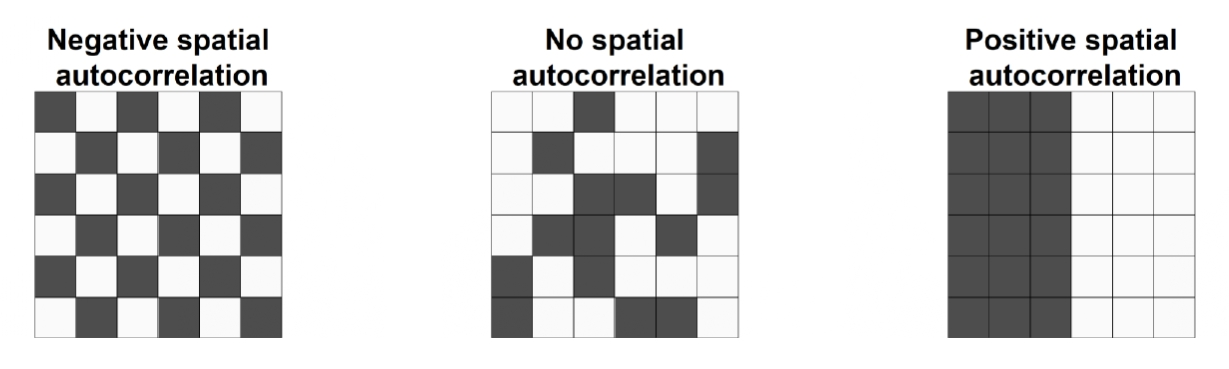
\includegraphics[keepaspectratio]{source/autocorrelation.jpg}}

}

\caption{\label{fig-autocorrelation}Examples of configurations of areas
showing different types of spatial autocorrelation}

\end{figure}%

To determine the significance of the Moran's I statistic, we employ the
Central Limit Theorem to calculate p-values based on a Z-score, allowing
us to test the following hypotheses:

\begin{itemize}
\tightlist
\item
  \(H_0: I = 0\) (no spatial autocorrelation),
\item
  \(H_1: I \neq 0\) (presence of spatial autocorrelation).
\end{itemize}

\subsection{Results}\label{sec-results}

\subsubsection{Exploratory Data
Analysis}\label{exploratory-data-analysis}

Figure~\ref{fig-sch} shows that mukims with higher schools count located
in the coastal region near South China Sea. As expected, majority of
mukims with high school count are in Brunei-Muara District (north-east
of mainland), the most populated and urban district in Brunei.

\begin{Shaded}
\begin{Highlighting}[]
\NormalTok{label\_sf }\OtherTok{\textless{}{-}}\NormalTok{ brn\_mkm\_sch\_sf }\SpecialCharTok{|\textgreater{}} 
  \FunctionTok{arrange}\NormalTok{(}\FunctionTok{desc}\NormalTok{(schools)) }\SpecialCharTok{|\textgreater{}} 
  \FunctionTok{slice\_head}\NormalTok{(}\AttributeTok{n =} \DecValTok{5}\NormalTok{) }\SpecialCharTok{|\textgreater{}} 
  \FunctionTok{mutate}\NormalTok{(}\AttributeTok{label =} \FunctionTok{paste0}\NormalTok{(mukim, }\StringTok{"}\SpecialCharTok{\textbackslash{}n}\StringTok{"}\NormalTok{, schools))}
\FunctionTok{ggplot}\NormalTok{() }\SpecialCharTok{+}
  \FunctionTok{geom\_sf}\NormalTok{(}\AttributeTok{data =}\NormalTok{ brn\_mkm\_sch\_sf, }\FunctionTok{aes}\NormalTok{(}\AttributeTok{fill =}\NormalTok{ schools)) }\SpecialCharTok{+}
  \FunctionTok{geom\_sf}\NormalTok{(}\AttributeTok{data =}\NormalTok{ mkm\_sf, }\AttributeTok{color=}\StringTok{"grey"}\NormalTok{, }\AttributeTok{alpha=}\DecValTok{0}\NormalTok{, }\AttributeTok{linewidth=}\FloatTok{0.7}\NormalTok{) }\SpecialCharTok{+}
  \FunctionTok{geom\_sf}\NormalTok{(}\AttributeTok{data =}\NormalTok{ dis\_sf, }\AttributeTok{color=}\StringTok{"red"}\NormalTok{, }\AttributeTok{alpha=}\DecValTok{0}\NormalTok{, }\AttributeTok{linewidth=}\FloatTok{0.5}\NormalTok{) }\SpecialCharTok{+}
\NormalTok{  ggrepel}\SpecialCharTok{::}\FunctionTok{geom\_label\_repel}\NormalTok{(}
    \AttributeTok{data =}\NormalTok{ label\_sf,}
    \FunctionTok{aes}\NormalTok{(}\AttributeTok{label =}\NormalTok{ label, }\AttributeTok{geometry =}\NormalTok{ geometry),}
    \AttributeTok{stat =} \StringTok{"sf\_coordinates"}\NormalTok{,}
    \AttributeTok{inherit.aes =} \ConstantTok{FALSE}\NormalTok{,}
    \AttributeTok{box.padding =} \DecValTok{1}\NormalTok{,}
    \AttributeTok{size =} \FloatTok{2.5}\NormalTok{,}
    \AttributeTok{alpha =} \FloatTok{0.7}\NormalTok{,}
    \AttributeTok{force=}\DecValTok{5}\NormalTok{,}
    \AttributeTok{max.overlaps =} \ConstantTok{Inf}
\NormalTok{  ) }\SpecialCharTok{+}
  \FunctionTok{scale\_fill\_viridis\_b}\NormalTok{(}
    \AttributeTok{option =} \StringTok{"E"}\NormalTok{,}
    \AttributeTok{direction =} \DecValTok{1}\NormalTok{,}
    \AttributeTok{name =} \StringTok{"School }\SpecialCharTok{\textbackslash{}n}\StringTok{Count"}\NormalTok{,}
    \AttributeTok{na.value =} \ConstantTok{NA}\NormalTok{,}
    \AttributeTok{breaks =} \FunctionTok{c}\NormalTok{(}\DecValTok{0}\NormalTok{,}\DecValTok{2}\NormalTok{,}\DecValTok{4}\NormalTok{,}\DecValTok{6}\NormalTok{,}\DecValTok{8}\NormalTok{)    }\CommentTok{\# Number of bins}
\NormalTok{  ) }\SpecialCharTok{+}
  \FunctionTok{labs}\NormalTok{(}\AttributeTok{x =} \ConstantTok{NULL}\NormalTok{, }\AttributeTok{y =} \ConstantTok{NULL}\NormalTok{) }\SpecialCharTok{+}
  \FunctionTok{theme\_minimal}\NormalTok{()}
\end{Highlighting}
\end{Shaded}

\begin{figure}[H]

\centering{

\pandocbounded{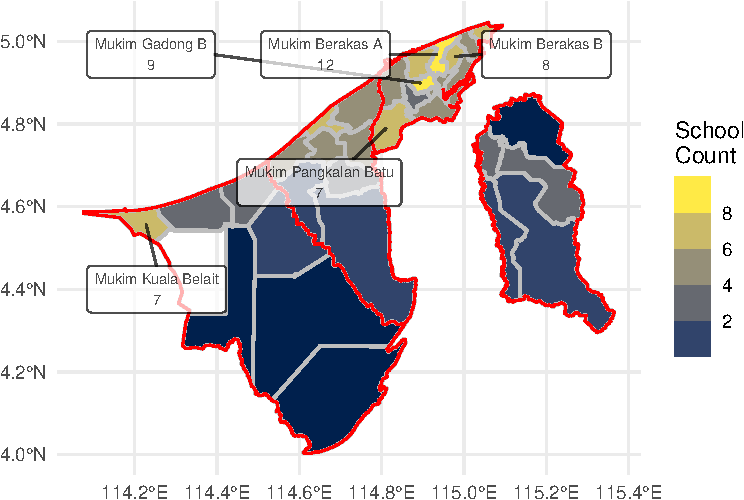
\includegraphics[keepaspectratio]{index_files/figure-pdf/fig-sch-1.pdf}}

}

\caption{\label{fig-sch}Choropleth Map of school count by mukim. Grey
boundaries denote mukim. Red boundaries are the 4 districts in Brunei.}

\end{figure}%

\subsubsection{Model}\label{sec-results-model}

The model results show that the intercept is estimated at
\(\hat{\beta}_0 = 1.077\), with a 95\% credible interval of
\((0.239, 1.894)\). The coefficient for population,
\(\beta_1 = -0.436\), with a 95\% credible interval of
\((-0.579, -0.295)\), indicates a statistically significant negative
relationship between population size and relative school abundance.
Specifically, for every 10,000 increase in population, the relative
abundance of schools decreases by approximately 35\%, since
\(\exp(-0.436) \approx 0.647\). In contrast, the covariates: mukim size
and house price are not statistically significant. The coefficient for
mukim size is \(\hat{\beta_2}=0.015\) (95\% CI: -0.002, 0.032), and for
house price is \(\hat{\beta_3}=-0.759\) (95\% CI: -3.174, 1.704).

The estimated relative abundance (RA) of schools across mukims
(Figure~\ref{fig-ra})vindicates lower values in the northern coastal
mukims, particularly in northern Brunei-Muara District, along the South
China Sea. Conversely, higher RA values appear inland, especially in
less densely populated regions.

To identify mukims with potentially inadequate school provision,
non-exceedence probabilities were computed for a threshold of
\(RA <0.7\). The analysis (Figure~\ref{fig-exc}) indicates that it is
highly likely that several mukims fall below this threshold, including
\textbf{Mukim Sengkurong, Mukim Gadong A, Mukim Gadong B, Mukim Berakas
B, and Mukim Mentiri}.

Lastly, the global Moran's I statistic of \(0.213\) (\(p<0.05\))
provides statistically significant evidence to reject the null
hypothesis of no spatial autocorrelation in the residuals.

\begin{Shaded}
\begin{Highlighting}[]
\NormalTok{label\_sf }\OtherTok{\textless{}{-}}\NormalTok{ brn\_mkm\_sch\_sf }\SpecialCharTok{|\textgreater{}} 
  \FunctionTok{filter}\NormalTok{(RA}\SpecialCharTok{!=}\DecValTok{0}\NormalTok{) }\SpecialCharTok{|\textgreater{}} 
  \FunctionTok{arrange}\NormalTok{(RA) }\SpecialCharTok{|\textgreater{}} 
  \FunctionTok{slice\_head}\NormalTok{(}\AttributeTok{n =} \DecValTok{5}\NormalTok{) }\SpecialCharTok{|\textgreater{}} 
  \FunctionTok{mutate}\NormalTok{(}\AttributeTok{label =} \FunctionTok{paste0}\NormalTok{(mukim, }\StringTok{"}\SpecialCharTok{\textbackslash{}n}\StringTok{"}\NormalTok{, }\FunctionTok{round}\NormalTok{(RA,}\DecValTok{2}\NormalTok{)))}
\FunctionTok{ggplot}\NormalTok{() }\SpecialCharTok{+}
  \FunctionTok{geom\_sf}\NormalTok{(}\AttributeTok{data =}\NormalTok{ brn\_mkm\_sch\_sf, }\FunctionTok{aes}\NormalTok{(}\AttributeTok{fill =}\NormalTok{ RA)) }\SpecialCharTok{+}
  \FunctionTok{geom\_sf}\NormalTok{(}\AttributeTok{data =}\NormalTok{ mkm\_sf, }\AttributeTok{color=}\StringTok{"grey"}\NormalTok{, }\AttributeTok{alpha=}\DecValTok{0}\NormalTok{, }\AttributeTok{linewidth=}\FloatTok{0.7}\NormalTok{) }\SpecialCharTok{+}
\NormalTok{  ggrepel}\SpecialCharTok{::}\FunctionTok{geom\_label\_repel}\NormalTok{(}
    \AttributeTok{data =}\NormalTok{ label\_sf,}
    \FunctionTok{aes}\NormalTok{(}\AttributeTok{label =}\NormalTok{ label, }\AttributeTok{geometry =}\NormalTok{ geometry),}
    \AttributeTok{stat =} \StringTok{"sf\_coordinates"}\NormalTok{,}
    \AttributeTok{inherit.aes =} \ConstantTok{FALSE}\NormalTok{,}
    \AttributeTok{box.padding =} \DecValTok{1}\NormalTok{,}
    \AttributeTok{size =} \DecValTok{3}\NormalTok{,}
    \AttributeTok{alpha =} \FloatTok{0.7}\NormalTok{,}
    \AttributeTok{force=}\DecValTok{5}\NormalTok{,}
    \AttributeTok{max.overlaps =} \ConstantTok{Inf}
\NormalTok{  ) }\SpecialCharTok{+}
  \FunctionTok{scale\_fill\_viridis\_b}\NormalTok{(}
    \AttributeTok{option =} \StringTok{"E"}\NormalTok{,}
    \AttributeTok{direction =} \SpecialCharTok{{-}}\DecValTok{1}\NormalTok{,}
    \AttributeTok{name =} \StringTok{"RA"}\NormalTok{,}
    \AttributeTok{na.value =} \ConstantTok{NA}\NormalTok{,}
    \AttributeTok{breaks =} \FunctionTok{c}\NormalTok{(}\DecValTok{0}\NormalTok{,}\DecValTok{1}\NormalTok{,}\DecValTok{2}\NormalTok{,}\DecValTok{3}\NormalTok{)    }\CommentTok{\# Number of bins}
\NormalTok{  ) }\SpecialCharTok{+}
  \FunctionTok{labs}\NormalTok{(}\AttributeTok{x =} \ConstantTok{NULL}\NormalTok{, }\AttributeTok{y =} \ConstantTok{NULL}\NormalTok{) }\SpecialCharTok{+}
  \FunctionTok{theme\_minimal}\NormalTok{()}
\end{Highlighting}
\end{Shaded}

\begin{figure}[H]

\centering{

\pandocbounded{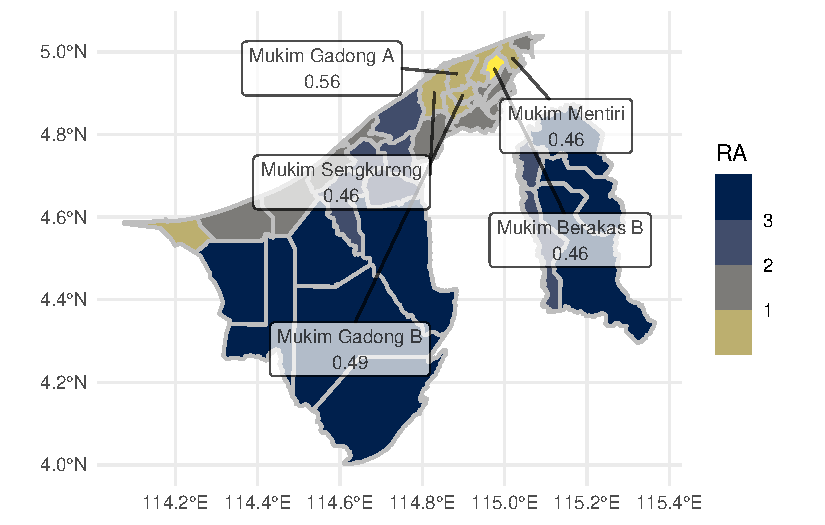
\includegraphics[keepaspectratio]{index_files/figure-pdf/fig-ra-1.pdf}}

}

\caption{\label{fig-ra}Relative Abudance of Schools in each mukim.}

\end{figure}%

\begin{Shaded}
\begin{Highlighting}[]
\NormalTok{brn\_mkm\_sch\_sf}\SpecialCharTok{$}\NormalTok{exc }\OtherTok{\textless{}{-}} \FunctionTok{sapply}\NormalTok{(res}\SpecialCharTok{$}\NormalTok{marginals.fitted.values,}
                    \AttributeTok{FUN =} \ControlFlowTok{function}\NormalTok{(marg)\{}\FunctionTok{inla.pmarginal}\NormalTok{(}\AttributeTok{q =} \FloatTok{0.7}\NormalTok{, }\AttributeTok{marginal =}\NormalTok{ marg)\})}

\NormalTok{label\_sf }\OtherTok{\textless{}{-}}\NormalTok{ brn\_mkm\_sch\_sf }\SpecialCharTok{|\textgreater{}} 
  \FunctionTok{arrange}\NormalTok{(}\FunctionTok{desc}\NormalTok{(exc)) }\SpecialCharTok{|\textgreater{}} 
  \FunctionTok{slice\_head}\NormalTok{(}\AttributeTok{n =} \DecValTok{6}\NormalTok{) }\SpecialCharTok{|\textgreater{}} 
  \FunctionTok{mutate}\NormalTok{(}\AttributeTok{label =} \FunctionTok{paste0}\NormalTok{(mukim, }\StringTok{"}\SpecialCharTok{\textbackslash{}n}\StringTok{"}\NormalTok{, }\FunctionTok{round}\NormalTok{(exc,}\DecValTok{2}\NormalTok{)))}
\FunctionTok{ggplot}\NormalTok{() }\SpecialCharTok{+}
  \FunctionTok{geom\_sf}\NormalTok{(}\AttributeTok{data =}\NormalTok{ brn\_mkm\_sch\_sf, }\FunctionTok{aes}\NormalTok{(}\AttributeTok{fill =}\NormalTok{ exc)) }\SpecialCharTok{+}
  \FunctionTok{geom\_sf}\NormalTok{(}\AttributeTok{data =}\NormalTok{ mkm\_sf, }\AttributeTok{color=}\StringTok{"grey"}\NormalTok{, }\AttributeTok{alpha=}\DecValTok{0}\NormalTok{, }\AttributeTok{linewidth=}\FloatTok{0.7}\NormalTok{) }\SpecialCharTok{+}
\NormalTok{  ggrepel}\SpecialCharTok{::}\FunctionTok{geom\_label\_repel}\NormalTok{(}
    \AttributeTok{data =}\NormalTok{ label\_sf,}
    \FunctionTok{aes}\NormalTok{(}\AttributeTok{label =}\NormalTok{ label, }\AttributeTok{geometry =}\NormalTok{ geometry),}
    \AttributeTok{stat =} \StringTok{"sf\_coordinates"}\NormalTok{,}
    \AttributeTok{inherit.aes =} \ConstantTok{FALSE}\NormalTok{,}
    \AttributeTok{box.padding =} \DecValTok{1}\NormalTok{,}
    \AttributeTok{size =} \DecValTok{3}\NormalTok{,}
    \AttributeTok{alpha =} \FloatTok{0.7}\NormalTok{,}
    \AttributeTok{force=}\DecValTok{5}\NormalTok{,}
    \AttributeTok{max.overlaps =} \ConstantTok{Inf}
\NormalTok{  ) }\SpecialCharTok{+}
  \FunctionTok{scale\_fill\_viridis\_b}\NormalTok{(}
    \AttributeTok{option =} \StringTok{"E"}\NormalTok{,}
    \AttributeTok{direction =} \DecValTok{1}\NormalTok{,}
    \AttributeTok{name =} \StringTok{"Non{-}exceedance }\SpecialCharTok{\textbackslash{}n}\StringTok{Probability }\SpecialCharTok{\textbackslash{}n}\StringTok{RA\textless{}0.7"}\NormalTok{,}
    \AttributeTok{na.value =} \ConstantTok{NA}\NormalTok{,}
    \AttributeTok{breaks =} \FunctionTok{c}\NormalTok{(}\DecValTok{0}\NormalTok{,}\FloatTok{0.25}\NormalTok{,}\FloatTok{0.5}\NormalTok{,}\FloatTok{0.75}\NormalTok{)    }\CommentTok{\# Number of bins}
\NormalTok{  ) }\SpecialCharTok{+}
  \FunctionTok{labs}\NormalTok{(}\AttributeTok{x =} \ConstantTok{NULL}\NormalTok{, }\AttributeTok{y =} \ConstantTok{NULL}\NormalTok{) }\SpecialCharTok{+}
  \FunctionTok{theme\_minimal}\NormalTok{()}
\end{Highlighting}
\end{Shaded}

\begin{figure}[H]

\centering{

\pandocbounded{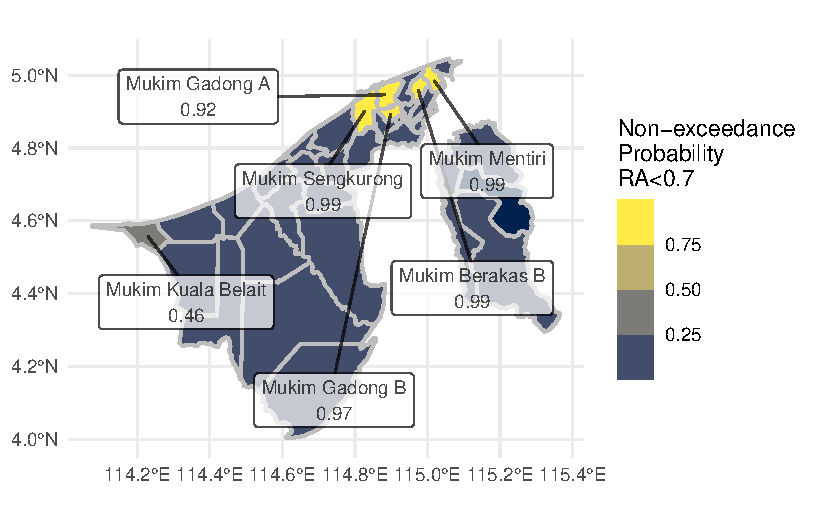
\includegraphics[keepaspectratio]{index_files/figure-pdf/fig-exc-1.pdf}}

}

\caption{\label{fig-exc}Mukims with non-exceedance probability of
Relative Abundance \textless{} 0.7}

\end{figure}%

\begin{Shaded}
\begin{Highlighting}[]
\NormalTok{fitted\_counts }\OtherTok{\textless{}{-}}\NormalTok{ brn\_mkm\_sch\_sf}\SpecialCharTok{$}\NormalTok{E }\SpecialCharTok{*}\NormalTok{ brn\_mkm\_sch\_sf}\SpecialCharTok{$}\NormalTok{RA}
\NormalTok{brn\_mkm\_sch\_sf}\SpecialCharTok{$}\NormalTok{residuals\_pearson }\OtherTok{\textless{}{-}}\NormalTok{ (brn\_mkm\_sch\_sf}\SpecialCharTok{$}\NormalTok{Y }\SpecialCharTok{{-}}\NormalTok{ fitted\_counts) }\SpecialCharTok{/} \FunctionTok{sqrt}\NormalTok{(fitted\_counts)}
\FunctionTok{ggplot}\NormalTok{() }\SpecialCharTok{+}
  \FunctionTok{geom\_sf}\NormalTok{(}\AttributeTok{data =}\NormalTok{ brn\_mkm\_sch\_sf, }\FunctionTok{aes}\NormalTok{(}\AttributeTok{fill =}\NormalTok{ residuals\_pearson)) }\SpecialCharTok{+}
  \FunctionTok{geom\_sf}\NormalTok{(}\AttributeTok{data =}\NormalTok{ mkm\_sf, }\AttributeTok{color=}\StringTok{"grey"}\NormalTok{, }\AttributeTok{alpha=}\DecValTok{0}\NormalTok{, }\AttributeTok{linewidth=}\FloatTok{0.7}\NormalTok{) }\SpecialCharTok{+}
  \FunctionTok{scale\_fill\_viridis\_b}\NormalTok{(}
    \AttributeTok{option =} \StringTok{"E"}\NormalTok{,}
    \AttributeTok{direction =} \DecValTok{1}\NormalTok{,}
    \AttributeTok{name =} \StringTok{"Residual"}\NormalTok{,}
    \AttributeTok{na.value =} \ConstantTok{NA}\NormalTok{,}
    \AttributeTok{n.breaks =} \DecValTok{6}    \CommentTok{\# Number of bins}
\NormalTok{  ) }\SpecialCharTok{+}
  \FunctionTok{labs}\NormalTok{(}\AttributeTok{x =} \ConstantTok{NULL}\NormalTok{, }\AttributeTok{y =} \ConstantTok{NULL}\NormalTok{) }\SpecialCharTok{+}
  \FunctionTok{theme\_minimal}\NormalTok{()}
\end{Highlighting}
\end{Shaded}

\begin{figure}[H]

\centering{

\pandocbounded{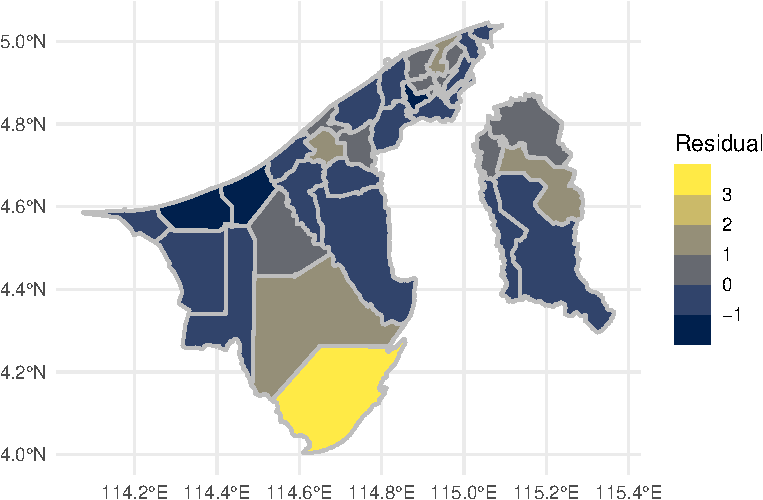
\includegraphics[keepaspectratio]{index_files/figure-pdf/fig-res-1.pdf}}

}

\caption{\label{fig-res}Spatial distribution of Pearson residuals from
the Poisson Bayesian model of school counts per mukim}

\end{figure}%

\subsection{Discussion}\label{discussion}

The results in Section~\ref{sec-results-model} offer insights into both
overall model performance and patterns of educational equity. Global
Moran's I statistic (0.213) is not substantially high (\textless0.3),
suggesting that the model captures most, but not all, of the residual
spatial dependence. This is illustrated in Figure~\ref{fig-res}, where
the variation in residual colors suggests a reasonably good fit, though
further improvement may be possible with additional spatial covariates
or refined random effects. The negative relationship between population
and school counts, as well as higher RA values in inland (rural) mukims
than coastal ares with larger population suggests that school
availability in rural mukims seem to be adequate, potentially due to
legacy planning policies or intentional efforts to ensure equitable
access in remote areas.

In contrast, urban and peri-urban mukims in the Brunei-Muara District,
the country's most densely populated and economically active region,
show signs of disparities in school access. Notably, the high
non-exceedance probability of \(RA < 0.7\) in \textbf{Mukim Sengkurong,
Gadong A \& B, Berakas B, and Mentiri} indicates that they have fewer
schools than expected relative to their population sizes. These
disparities highlight areas that may be underinvested in educational
infrastructure, warranting closer policy attention.

Importantly, these mukims are also encompass several new government
housing developments, such as Perpindahan Lugu and Perpindahan Tanah
Jambu. This suggests a potential planning gap, where population is
increasing due to housing developments, but educational infrastructure
has not yet caught up.

However, inspection of Figure~\ref{fig-sch} reveals that these areas
have a similar number of schools compared to their neighboring mukims.
This suggests that while the absolute number of schools may not be
unusually low, the rapid increase in population within these new housing
areas may have outpaced school capacity, leading to a situation where
demand exceeds supply within these specific zones.

Nevertheless, this situation represents a strategic opportunity.
Prioritizing school construction in these fast-growing neighborhoods
could significantly improve access to education, reduce commute times,
lower transportation costs, and enhance the overall quality of life for
residents. Locating schools closer to homes supports national goals
related to sustainable urban development, walkability, and equity in
public services.

\subsubsection{Limitations}\label{limitations}

This study is limited to public schools, excluding private and
international institutions that may affect school availability in some
areas. The data is from 2018, potentially missing recent changes,
especially in fast-growing neighborhoods. Next, our model used the
general population data and is not age-standardized, are important for
demand estimation. Housing price was used as a proxy for socioeconomic
status, but data relies on listing prices, which may not reflect actual
market values due to negotiation factors. In some areas, price data was
also simulated, introducing further uncertainty.

\subsection{Conclusions}\label{sec-conc}

In summary, our model reveals a negative relationship between population
size and relative school abundance, suggesting urban areas have fewer
schools per capita than rural ones. Several mukims in the Brunei-Muara
District, including Sengkurong, Gadong A \& B, Berakas B, and Mentiri,
appear to have fewer schools than expected, despite ongoing population
growth driven by new housing developments. While total school counts may
seem adequate, local demand in these areas may exceed capacity.
Addressing this gap offers a strategic opportunity to improve access,
reduce travel time, and support equitable urban planning.

\subsection*{References}\label{references}
\addcontentsline{toc}{subsection}{References}

\phantomsection\label{refs}
\begin{CSLReferences}{1}{0}
\bibitem[\citeproctext]{ref-abdul2021development}
Abdul Latif, Siti Norhedayah, Rohani Matzin, and Aurelia Escoto-Kemp.
2021. {``The Development and Growth of Inclusive Education in Brunei
Darussalam.''} \emph{Globalisation, Education, and Reform in Brunei
Darussalam}, 151--75. \url{https://doi.org/10.1007/978-3-030-77119-5_8}.

\bibitem[\citeproctext]{ref-UNGA2015transform}
Assembly, United Nations General. 2015. {``Transforming Our World: The
2030 Agenda for Sustainable Development.''}
\url{https://sustainabledevelopment.un.org/post2015/transformingourworld}.

\bibitem[\citeproctext]{ref-GovernmentBruneiNDwawasan}
Brunei Darussalam, Government of. 2020. {``Brunei Darussalam Long-Term
Development Plan. Wawasan Brunei 2035.''}

\bibitem[\citeproctext]{ref-ebil2023overview}
Ebil, Syazana, and Masitah Shahrill. 2023. {``Overview of Education in
Brunei Darussalam.''} In \emph{International Handbook on Education in
South East Asia}, 1--21. Springer.
\url{https://doi.org/10.1007/978-981-16-8136-3_46-1}.

\bibitem[\citeproctext]{ref-bruneimap}
Jamil, Haziq. 2025. \emph{Bruneimap: {M}aps and {S}patial {D}ata of
{B}runei ({R} Package Version 0.3.1.9001)}.
\url{https://bruneiverse.github.io/bruneimap/}.

\bibitem[\citeproctext]{ref-jamil2025archives}
Jamil, Haziq, Amira Barizah Noorosmawie, Hafeezul Waezz Rabu, and Lutfi
Abdul Razak. 2025. {``From {Archives} to {AI:} {Residential} {Property}
{Data} {Across} {Three} {Decades} in {Brunei} {Darussalam}.''}
\emph{Data in Brief}, March.
\url{https://doi.org/10.1016/j.dib.2025.111505}.

\bibitem[\citeproctext]{ref-mohamad2018towards}
Mohamad, Hanapi, Rosyati M Yaakub, Emma Claire Pearson, and Jennifer Tan
Poh Sim. 2018. {``Towards Wawasan Brunei 2035: Early Childhood Education
and Development in Brunei Darussalam.''} \emph{International Handbook of
Early Childhood Education}, 551--67.
\url{https://doi.org/10.1007/978-94-024-0927-7_25}.

\bibitem[\citeproctext]{ref-salbrina2024education}
Salbrina, Sharbawi, David Deterding, and Mohamad Nur Raihan. 2024.
{``Education in Brunei.''} In \emph{Brunei English: A New Variety in a
Multilingual Society}, 17--32. Springer.
\url{https://doi.org/10.1007/978-3-031-60303-7_2}.

\end{CSLReferences}




\end{document}
